\documentclass[12pt,a4paper]{article}

% Paquetes básicos
\usepackage[utf8]{inputenc}
\usepackage[T1]{fontenc}
\usepackage[spanish]{babel}
\usepackage{amsmath, amssymb}
\usepackage{siunitx} % Ángulos
\usepackage{graphicx}
\usepackage{float}
\usepackage{geometry}
\usepackage{xcolor}
\geometry{margin=2.5cm}
\usepackage{array}
\usepackage{longtable}
\usepackage{hyperref}
\usepackage{caption}
\usepackage{subcaption}
\usepackage{setspace}
\usepackage{multirow}
\usepackage{minted}  % Códigos
\usepackage{gensymb} % Grados: "°"
\usepackage[backend=biber, style=ieee]{biblatex}
\usepackage{csquotes}
\usepackage{booktabs}
\addbibresource{Bibliografía.bib}
\graphicspath{{Figuras/}}
\onehalfspacing
\hypersetup{
    colorlinks  = true,
    linkcolor   = blue,    
    citecolor   = blue,
    urlcolor    = blue,
    filecolor   = blue
}


\begin{document}       
\renewcommand{\figureautorefname}{Fig.}
\renewcommand{\tableautorefname}{Tab.}
\renewcommand{\equationautorefname}{Ec.}


% Carátula personalizada
\begin{titlepage}
    \centering
    
\includegraphics[width=0.7\textwidth]{Marvell Logo.png}\\[1.5cm]

    {\Large \textbf{PROGRAMA DE FORMACIÓN MARVELL} \\[0.5cm]}
    {\Large Diseño Digital para Sistemas DSP} \\[0.5cm]

    \rule{\textwidth}{0.5pt} \\[0.5cm]
    {\Large \textbf{Ejercicios Módulo 4: Circuitos Aritméticos I} \\[0.3cm]}
    \rule{\textwidth}{0.5pt} \\[1cm]
    
\vfill
\begin{tabular}{l l}
    \textbf{Profesor:} & Del Barco, Martín.\\
    \\[0.5cm]
    \textbf{Alumnos:} & Monja, Ernesto Joaquín\\
                      & Zúñiga, Guillermo Rubén Darío\\
\end{tabular} \\[5cm]
\vfill
{\centering Año 2026 \par}

\end{titlepage}



% Índice
\tableofcontents
\newpage



\section{Introducción}                                              \label{sec_1}
El presente informe detalla el diseño, implementación y verificación de diversos circuitos aritméticos fundamentales para el procesamiento digital de señales (\textit{DSP}), desarrollados en lenguaje \textit{SystemVerilog}. A lo largo del documento se exploran distintas arquitecturas de sumadores —Ripple Carry Adder (\textit{RCA}), Carry-Lookahead Adder (\textit{CLA}) y Carry Select Adder (\textit{CSLA})— así como de multiplicadores —secuencial \textit{Shift and Add}, \textit{Array} combinacional y \textit{Booth Radix-2}—. El objetivo principal es analizar y contrastar el desempeño teórico y práctico de cada topología en términos de retardo temporal, uso de área lógica, latencia y \textit{throughput}, validando su correcto funcionamiento mediante simulaciones exhaustivas en entornos de \textit{testbench}.



\section{Desarrollo}                                                \label{sec_2}
\subsection{RCA \textit{N-bit} Parametrizable}                      \label{sec_2.1}
Se implementó un Ripple Carry Adder (\textit{RCA}) parametrizable de $N$ bits utilizando una estructura puramente jerárquica y generativa en \textit{SystemVerilog}. La arquitectura se basa en la instanciación concatenada de módulos \textit{Full-Adder} mediante una sentencia \textit{generate-for}. Cada bloque procesa dos bits de entrada ($a[i]$, $b[i]$) y el acarreo entrante ($c[i]$), produciendo la suma parcial ($s[i]$) y el acarreo saliente ($c[i+1]$).

Dado que la topología encadena \textit{adders} completos de $1$ bit de forma lineal, la cantidad total de bloques \textit{Full-Adder} requeridos escala proporcionalmente con el ancho de palabra $N$:
\begin{equation}
    \text{Cantidad de FAs} = N
    \label{eq_1}
\end{equation}

Para las distintas configuraciones evaluadas, la cantidad de celdas utilizadas es:
\begin{itemize}
    \item $N = 4$:  $4$ \textit{Full-Adders}
    \item $N = 8$:  $8$ \textit{Full-Adders} (configuración por defecto)
    \item $N = 16$: $16$ \textit{Full-Adders}
    \item $N = 32$: $32$ \textit{Full-Adders}
\end{itemize}

El camino crítico del \textit{RCA} está determinado por la propagación en serie del acarreo a lo largo de los $N$ estadios. El retardo total de propagación $t_{RCA}$ viene dado por la \autoref{eq_2}. \cite{b1}
\begin{equation}
    t_{RCA} = t_{cin \to cout\_FA0} + (N - 2) \cdot t_{carry\_step} + t_{cin \to sum\_FAN-1} \approx \mathcal{O}(N)
    \label{eq_2}
\end{equation}

El peor caso se produce cuando una transición en los bits menos significativos ($a[0], b[0]$ o $cin$) requiere propagar el acarreo desde la primera posición hasta la última (por ejemplo, al sumar $0xFE_{h} + 0x01_{h}$ con $cin = 0$). Esta dependencia lineal ($\mathcal{O}(N)$) representa la principal limitación de velocidad del sumador \textit{RCA} para anchos de palabra grandes.

A continuación se presenta en la \autoref{tab:tab_1}, la relación entre el número de bits $N$ y el retardo relativo estimado acumulado en la cadena de acarreo:
\begin{table}[H]
    \centering
    \begin{tabular}{|c|c|c|} \hline
        \textbf{Ancho de palabra ($N$)} & \textbf{Cantidad de \textit{FAs}} & \textbf{Retardo relativo de acarreo ($\propto N$)} \\ \hline
        4 bits  & 4  & $4 \, \Delta t$ \\ \hline
        8 bits  & 8  & $8 \, \Delta t$ \\ \hline
        16 bits & 16 & $16 \, \Delta t$ \\ \hline
        32 bits & 32 & $32 \, \Delta t$ \\ \hline
    \end{tabular}
    \caption{Relación de retardo de propagación según el ancho de palabra $N$.}
    \label{tab:tab_1}
\end{table}

La verificación funcional se llevó a cabo mediante el \textit{testbench} auto-chequeable (\texttt{tb\_rca.sv}), el cual evaluó con éxito un total de 503 vectores de prueba con resolución de tiempo de $1 \, [ns] / 1 \, [ps]$:
\begin{itemize}
    \item \underline{Borde Inferior:} $0 + 0 + 0 = 0$ ($cout = 0$).
    \item \underline{Borde Superior:} $(2^{N} - 1) + (2^{N} - 1) + 0 = 2^{N + 1} - 2$ ($cout = 1$).
    \item \underline{Generación de Carry-out:} $0xFF_{h} + 0x01_{h} = 0x100_{h}$ ($cout = 1, s = 0$).
    \item \underline{Pruebas Aleatorias:} 500 estimulaciones pseudo-aleatorias con $cin \in \{0, 1\}$.
\end{itemize}

La simulación concluyó exitosamente a los $5.03 \, [\mu s]$ sin reportar inconsistencias tal como lo muestra la \autoref{fig:fig_1} y la \autoref{fig:fig_2}.
\begin{figure}[h]
    \centering
    
\includegraphics[width=0.5\linewidth]{Figura 1.png}
    \caption{Salida de consola.}
    \label{fig:fig_1}
\end{figure}
\begin{figure}[h]
    \centering
    
\includegraphics[width=1.05\linewidth]{Figura 2.png}
    \caption{Salida de \textit{GTKwave} donde se observa que la variable \texttt{errors} es siempre $0$.}
    \label{fig:fig_2}
\end{figure}



\subsection{\emph{Carry-Lookahead Adder} (CLA) Jerárquico}           \label{sec_2.2}
El \textit{CLA} define el concepto de \emph{generate} y \emph{propagate}, y utilizando las \autoref{eq:generate}, \autoref{eq:propagate} y \autoref{eq:carry}, establece el carry del bit siguiente como una relación entre el generate, propagate y el carry anterior.
\begin{equation}
    g_i = a_i \cdot b_i
    \label{eq:generate}
\end{equation}

\begin{equation}
    p_i = a_i \oplus b_i
    \label{eq:propagate}
\end{equation}

\begin{equation} 
    c_{i+1} = g_i + p_i \cdot c_i
    \label{eq:carry}
\end{equation}

La arquitectura de un \textit{CLA} de $4$ bits se muestra en la \autoref{fig:cla_4bits_esq}, consiste en $4$ \textit{Full-Adders} y una lógica que procesa el generate y el propagate. Este \textit{CLA} puede encadenarse para formar un sumador más grande, como se muestra en la \autoref{fig:cla_jerarquico_esq}.
\begin{figure}[H]
    \centering
    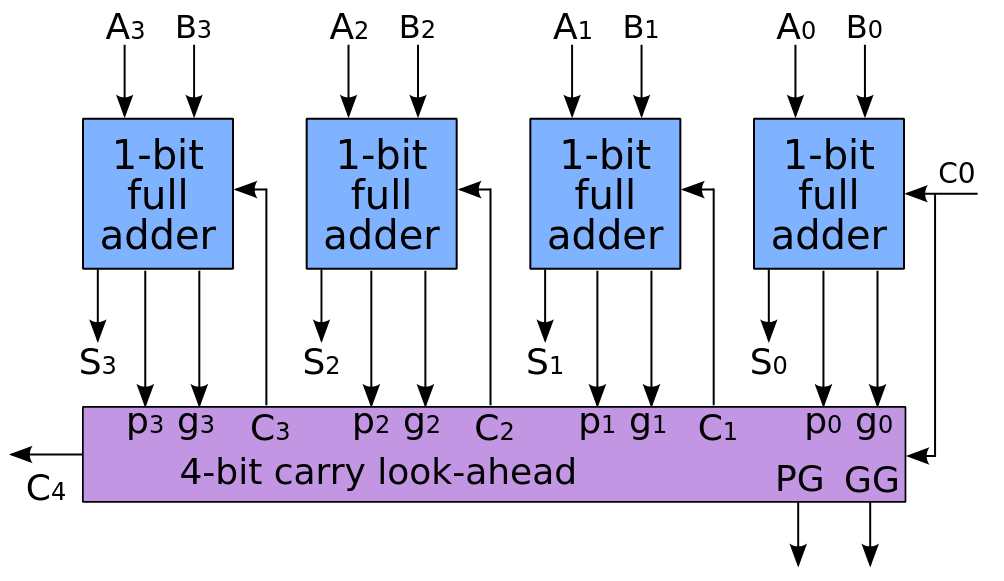
\includegraphics[width=0.6\linewidth]{Figuras/cla_4bits_esq.png}
    \caption{Arquitectura de un \textit{CLA} de $4$ bits.}
    \label{fig:cla_4bits_esq}
\end{figure}

\begin{figure}[H]
    \centering
    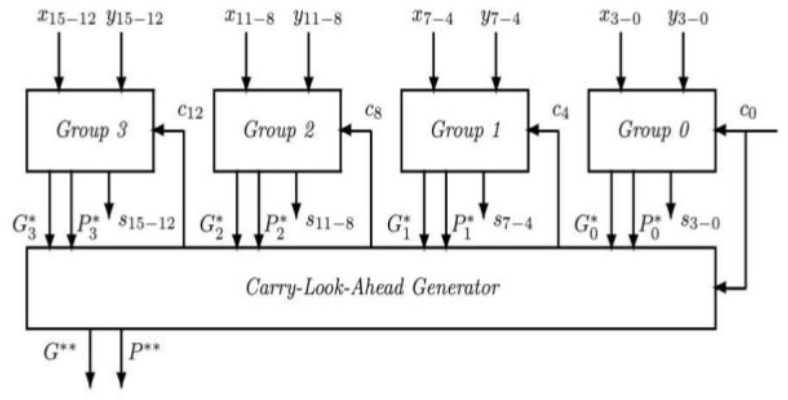
\includegraphics[width=0.7\linewidth]{Figuras/cla_jerarquico_esq.png}
    \caption{Arquitectura de un \textit{CLA} de $16$ bits.}
    \label{fig:cla_jerarquico_esq}
\end{figure}

Se implementó un \textit{CLA} de $4$ bits con estas ecuaciones explícitas, luego se encadenaron $4$ de estos módulos para formar un \textit{CLA} jerárquico de $16$ bits. De este modo, se esperó optimizar bastante el \textit{delay} entre compuertas ya que se diseñó en el módulo top una lógica de \textit{CLA} inter-bloque.

A este módulo de $16$ bits se lo verificó con un testbench que inyecta determinados casos de borde y otros 1000 casos aleatorios, para luego comparar los resultados con un modelo de suma ideal. Los resultados se muestran en la \autoref{fig:cla_print} y la \autoref{fig:cla_wave}.
\begin{figure}[H]
    \centering
    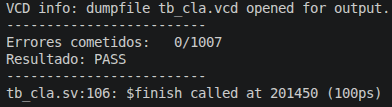
\includegraphics[width=0.5\linewidth]{cla_print.png}
    \caption{Resultado de la comparación con el golden model.}
    \label{fig:cla_print}
\end{figure}

\begin{figure}[H]
    \centering
    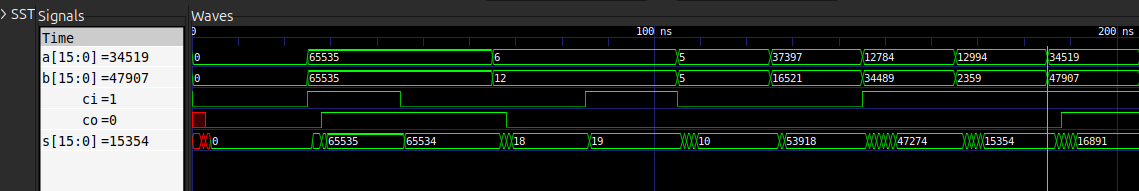
\includegraphics[width=\linewidth]{cla_wave.png}
    \caption{Porción de la forma de onda obtenida.}
    \label{fig:cla_wave}
\end{figure}

Se puede observar pequeñas variaciones cuando se modifica la entrada, y esto es porque se modeló un \textit{delay} de $1 \, [ns]$ para cada compuerta lógica. Esto sirvió para luego hacer la comparación con un \textit{RCA} de $16$ bits. Si se busca el caso con el mayor \textit{delay} (véase la \autoref{fig:cla_delay}), se observa que el máximo retardo que tiene este diseño es de $8$ gates.
\begin{figure}[H]
    \centering
    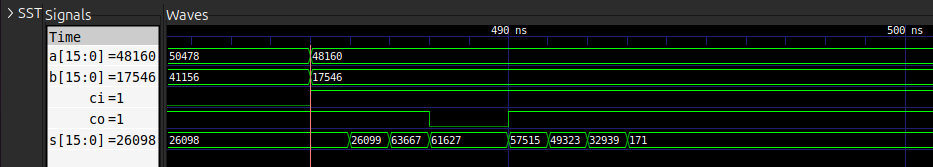
\includegraphics[width=\linewidth]{cla_delay.png}
    \caption{Forma de onda de la transición con \textit{delay} de 8 compuertas.}
    \label{fig:cla_delay}
\end{figure}

Se modeló un retardo en el full adder del RCA de la sección anterior para realizar la comparación en el peor caso. En la \autoref{fig:rca_delay} se puede observar un delay de 16 compuestas, que coincide con lo esperado teóricamente. Luego, se compararon los diseños de 4 bits, donde la \autoref{tab:rca_cla} muestra los resultados. Para 4 bits no se observó diferencias, pero para 16 bits el CLA es mucho más rápido, ya que posee la lógica que procesa todos los carry en paralelo, en lugar de esperar al carry del bit anterior para realizar la suma de los bits actuales.
\begin{figure}[H]
    \centering
    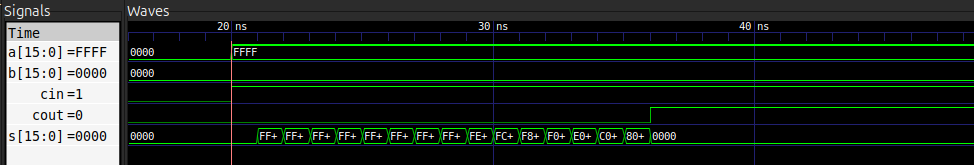
\includegraphics[width=\linewidth]{Figuras/rca_delay.png}
    \caption{Forma de onda de la transición en el RCA, con \textit{delay} de 16 compuertas.}
    \label{fig:rca_delay}
\end{figure}

\begin{table}[H]
    \centering
    \begin{tabular}{ccc}
    \hline
    $N_{bits}$ &  Delay RCA & Delay CLA  \\ \hline
    4      & 4 & 4 \\
    16      & 16 & 8 \\ \hline
    \end{tabular}
    \caption{Comparación de retardos entre RCA y CLA (en número de compuertas).}
    \label{tab:rca_cla}
\end{table}

\subsection{\textit{CSLA} por bloques de $4$ bits (opcional)}        \label{sec_2.3}
Se diseñó un sumador Carry Select Adder (\textit{CSLA}) de $16$ bits estructurado en $4$ bloques funcionales de $4$ bits cada uno. El principio de funcionamiento de esta arquitectura radica en el cálculo especulativo: mientras el primer bloque computa la suma real a partir del acarreo de entrada general ($cin$), los bloques sucesivos calculan simultáneamente $2$ posibles resultados (uno asumiendo $cin = 0$ y otro asumiendo $cin = 1$). Una vez que el acarreo del bloque anterior se estabiliza, se utiliza para comandar un multiplexor $2:1$ que selecciona el resultado correcto.

El diseño se modularizó en $2$ archivos principales:
\begin{itemize}
    \item \texttt{rca4.sv}: Un sumador de acarreo propagado de $4$ bits, utilizado como bloque base.
    \item \texttt{csla16.sv}: El módulo superior que instancia un \textit{RCA} simple para los bits $[3:0]$, y un par de \textit{RCA} redundantes junto con multiplexores para los bloques $[7:4]$, $[11:8]$ y $[15:12]$.
\end{itemize}

Al compilar ambos archivos, obtenemos las salidas mostradas en la \autoref{fig:fig_3} y \autoref{fig:fig_4}.
\begin{figure}[h]
    \centering
    
\includegraphics[width=0.5\linewidth]{Figuras/Figura 3.png}
    \caption{Salida de consola.}
    \label{fig:fig_3}
\end{figure}
\begin{figure}[h]
    \centering
    
\includegraphics[width=1.05\linewidth]{Figuras/Figura 4.png}
    \caption{Salida de \textit{GTKwave} donde se observa que la variable \texttt{errors} es siempre $0$.}
    \label{fig:fig_4}
\end{figure}

A continuación se presenta en la \autoref{tab:tab_2}, un análisis cualitativo del área y el retardo teórico (asumiendo compuertas ideales) para sumadores de $16$ bits:
\begingroup
\footnotesize
\begin{longtable}
    {|>{\centering\arraybackslash}m{3.5cm}
     |>{\centering\arraybackslash}m{3.5cm}
     |>{\centering\arraybackslash}m{3.5cm}
     |>{\centering\arraybackslash}m{3.5cm}|} \hline
    \textbf{Métrica} & \textbf{RCA} & \textbf{CLA} & \textbf{CSLA} \\ \hline
    \endfirsthead
    
    \multicolumn{4}{c}{\textit{Continuación de la página anterior}} \\ \hline
    \textbf{Métrica} & \textbf{RCA} & \textbf{CLA} & \textbf{CSLA} \\ \hline
    \endhead
    
    \hline 
    \textbf{Métrica} & \textbf{RCA} & \textbf{CLA} & \textbf{CSLA} \\ \hline
    \endfoot
    
    \hline
    \caption{Comparativa Teórica: CSLA, CLA y RCA (16 bits).}
    \label{tab:tab_2} \\
    \endlastfoot

    \textbf{Área (Hardware)} & Baja ($\approx 16$ \textit{FAs}) & Alta (Lógica Lookahead) & Alta ($\approx 28$ \textit{FAs + MUXes}) \\ \hline
    
    \textbf{Delay Teórico} & $\mathcal{O}(N)$ & $\mathcal{O}(\log_2 N)$ & $\mathcal{O}(\sqrt{N})$ (bloques variables) / Constante por \textit{MUX} \\ \hline
    
    \textbf{Camino Crítico} & Ripple por $16$ bits & Árbol de Lookahead & Ripple de $4$ bits + $3$ \textit{MUXes} \\ \hline
\end{longtable}
\endgroup

Si el objetivo principal de diseño es alcanzar una frecuencia máxima de operación alta ($F_{max}$), el \textit{CLA} suele ser la mejor opción, ya que su retardo logarítmico escala de forma muy eficiente, aunque su implementación en celdas estándar puede requerir un \textit{fan-in/fan-out} considerable. 

Por otro lado, el \textit{CSLA} elimina la propagación (\textit{ripple}) inter-bloque delegando el retardo a una cadena de multiplexores rápidos, lo cual mejora drásticamente el tiempo de ciclo frente a un \textit{RCA} puro a costa de casi duplicar el área del sumador. En tecnologías modernas donde el coste de los multiplexores es muy bajo, el \textit{CSLA} ofrece un balance excelente entre simplicidad de diseño (reutilización de bloques \textit{RCA}) y alta velocidad.




\subsection{Multiplicador Secuencial \emph{Shift and Add}}           \label{sec_2.4}
En sistemas donde el bajo consumo y el área es más prioritario que la latencia o el \textit{throughput}, se utiliza una arquitectura secuencial que reutiliza sumadores y registros denominada \textit{Shift and Add Multiplier}. El concepto de funcionamiento se muestra en la \autoref{fig:shiftadd_ejemplo}.

Se armó un módulo en \textit{SystemVerilog} que consiste en una \textit{FSM} y un multiplicador \textit{Shift and Add}. Esta máquina de estados permite controlar el multiplicador, habilitándolo solo cuando sea necesario y conociendo cuando se completó la operación, todo esto con las banderas \emph{start} y \emph{done}. El diagrama de estados se muestra en la \autoref{fig:shiftadd_fsm}.
\begin{figure}[H]
    \centering
    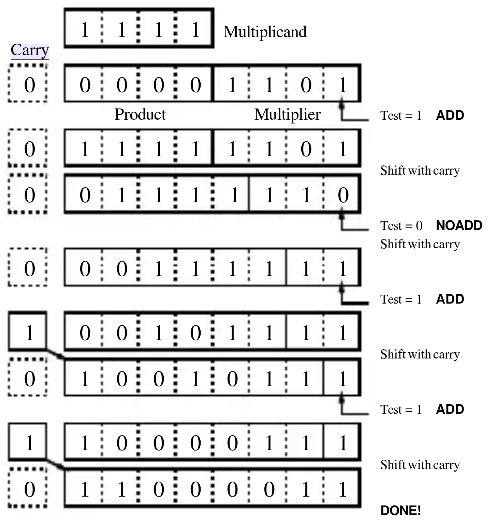
\includegraphics[width=0.5\linewidth]{shiftadd_ejemplo.png}
    \caption{Ejemplo del método \textit{Shift and Add} con $4$ bits de entrada.}
    \label{fig:shiftadd_ejemplo}
\end{figure}

\begin{figure}[H]
    \centering
    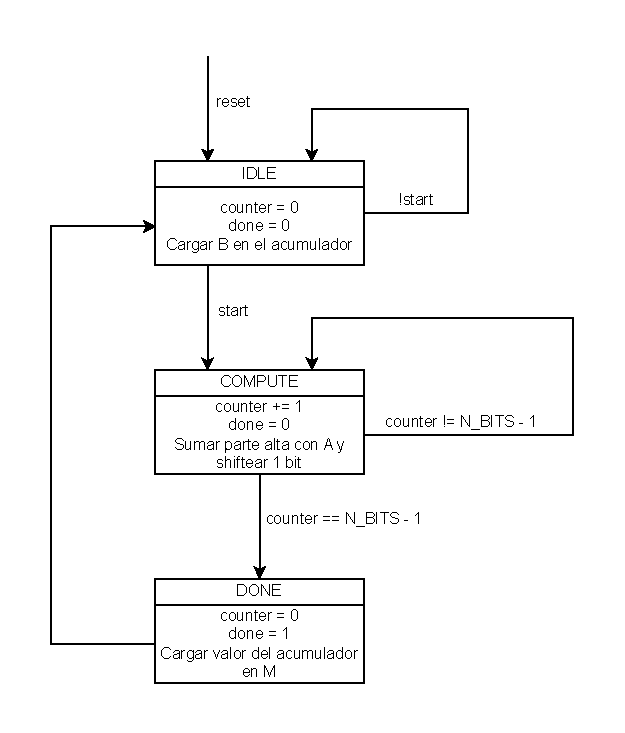
\includegraphics[width=0.7\linewidth]{shiftadd_fsm.pdf}
    \caption{Diagrama de estados del multiplicador Shift and Add.}
    \label{fig:shiftadd_fsm}
\end{figure}

Este módulo se verificó en un \textit{testbench} con poco mas de $200$ casos y comparando con el resultado de la multiplicación directa. El resultado en la \autoref{fig:shiftadd_print} demuestra que el módulo realiza correctamente la operación. Como se puede observar en la forma de onda de la \autoref{fig:shiftadd_wave}, la latencia en la recepción del dato es de $10$ flancos de reloj, pero el multiplicador en sí tarda 8 ciclos, como se puede observar en el contador \emph{counter} interno. Si el multiplicador tiene latencia de 8 ciclos, entonces se puede decir que el \textit{throughput} en este caso es de $1/8 = 0.125$.
\begin{figure}[H]
    \centering
    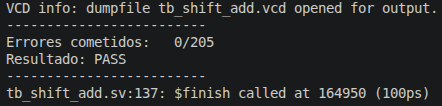
\includegraphics[width=0.6\linewidth]{shiftadd_print.png}
    \caption{Resultado impreso de la simulación.}
    \label{fig:shiftadd_print}
\end{figure}

\begin{figure}[H]
    \centering
    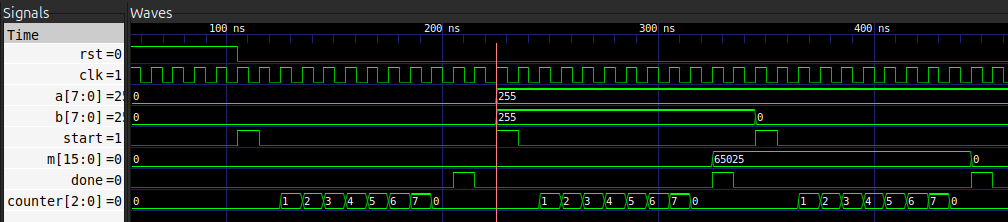
\includegraphics[width=\linewidth]{shiftadd_wave.png}
    \caption{Formas de onda del diseño.}
    \label{fig:shiftadd_wave}
\end{figure}

A comparación con otras arquitecturas, se puede ver que la cantidad de ciclos a esperar por el resultado es bastante alta, pero el uso de recursos a la hora de sintetizarlo es mucho menor. Es por esto que existen aplicaciones que requieren este método, como lo son los microcontroladores y el \textit{IoT}.

% area reportada por yosys:    Chip area for module '\shift_add': 2071.987200



\subsection{Array Multiplier $8 \times 8$ (combinacional)}           \label{sec_2.5}
Se implementó un multiplicador unsigned combinacional de $8 \times 8$ bits utilizando una matriz de suma de acarreos conservados (\textit{CSA}) y una fila final de propagación de acarreos (\textit{CPA}).

La estructura del módulo se divide en tres partes principales:
\begin{itemize}
    \item \underline{Generación de Productos Parciales (\textit{PP}):} Una matriz de $8 \times 8$ compuertas \textit{AND} ($64$ compuertas en total) que generan todos los bits de productos parciales de forma paralela.
    \item \underline{Matriz de Reducción (\textit{CSA}):} $7$ filas compuestas por $8$ \textit{Full-Adders} cada una ($56$ \textit{FAs} en total). En esta etapa, los acarreos no se propagan horizontalmente dentro de la misma fila, sino que se transmiten verticalmente hacia la fila inferior.
    \item \underline{Fila Final de Suma (\textit{CPA}):} Una fila de $8$ \textit{Full-Adders} configurados como un Ripple Carry Adder (\textit{RCA}) para sumar los bits acumulados y los acarreos restantes de la matriz CSA, entregando el resultado final de $16$ bits.
\end{itemize}

El módulo fue verificado exhaustivamente mediante el testbench \texttt{tb\_array\_mul.sv}, evaluando las $256 \times 256 = 65.536$ combinaciones posibles de las entradas. La simulación completó sin errores de coincidencia respecto al resultado esperado del *host* tal como muestran la \autoref{fig:fig_5} y la \autoref{fig:fig_6}.
\begin{figure}[H]
    \centering
    
\includegraphics[width=0.5\linewidth]{Figuras/Figura 5.png}
    \caption{Salida de consola.}
    \label{fig:fig_5}
\end{figure}
\begin{figure}[H]
    \centering
    
\includegraphics[width=1.05\linewidth]{Figuras/Figura 6.png}
    \caption{Salida de \textit{GTKwave} donde se observa que la variable \texttt{errors} es siempre $0$.}
    \label{fig:fig_6}
\end{figure}


El camino crítico ($T_{crit}$) está determinado por la propagación de las señales a través del arreglo: el retardo de una compuerta \textit{AND} inicial, la trayectoria diagonal/vertical a lo largo de las $7$ etapas \textit{CSA}, y la propagación horizontal completa en el sumador final (\textit{CPA}) de $8$ bits esta dada según la \autoref{eq_6}. \cite{b2}
\begin{equation}
    T_{\text{crit}} = \tau_{\text{AND}} + (N - 1) \cdot \tau_{\text{FA}} + N \cdot \tau_{\text{FA\_carry}} = \tau_{\text{AND}} + 15 \cdot \tau_{\text{FA}}
    \label{eq_6}
\end{equation}

En total, la solución implementa \textbf{64 Full Adders} ($56$ en la matriz \textit{CSA} + $8$ en la fila final \textit{CPA}) y \textbf{64 compuertas AND}. En la \autoref{tab:tab_3} se sintetiza la comparación de este diseño frente a la alternativa secuencial del Ejercicio $4$ desarrollado en la \autoref{sec_2.4} y la inferencia directa en \textit{RTL}.

Podemos entonces realizar la siguiente comparación:
\begin{itemize}
    \item \underline{Array vs. Secuencial:} El multiplicador matricial maximiza el \textit{throughput} procesando una operación completa por pulso sin requerir registros ni señal de reloj. No obstante, el costo en área aumenta significativamente al requerir \textit{64 FAs} en comparación con el único sumador de 8 bits.
    
    \item \underline{Array vs. RTL (\texttt{*}):} Aunque el multiplicador matricial elimina el ciclo de reloj, su retardo combinacional crece de forma lineal $\mathcal{O}(N)$ debido a la propagación del acarreo. Al inferir el operador \texttt{*}, la herramienta de síntesis suele utilizar estructuras optimizadas como árboles de \textit{Wallace/Dadda} con retardo logarítmico $\mathcal{O}(\log_2 N)$ o mapear directamente el cálculo a bloques \textit{DSP} nativos de la \textit{FPGA}, logrando una frecuencia máxima ($f_{max}$) superior.
\end{itemize}

\begingroup
\footnotesize
\begin{longtable}
    {|>{\centering\arraybackslash}m{3.5cm}
     |>{\centering\arraybackslash}m{3.5cm}
     |>{\centering\arraybackslash}m{3.5cm}
     |>{\centering\arraybackslash}m{3.5cm}|} \hline
    \textbf{Métrica} & \textbf{Secuencial} & \textbf{Array} & \textbf{RTL Directo \newline (\texttt{a * b})} \\ \hline
    \endfirsthead
    
    \multicolumn{4}{c}{\textit{Continuación de la página anterior}} \\ \hline
    \textbf{Métrica} & \textbf{Secuencial} & \textbf{Array} & \textbf{RTL Directo \newline (\texttt{a * b})} \\ \hline
    \endhead
    
    \hline 
    \textbf{Métrica} & \textbf{Secuencial} & \textbf{Array} & \textbf{RTL Directo \newline (\texttt{a * b})} \\ \hline
    \endfoot
    
    \hline
    \caption{Comparativa entre arquitecturas de multiplicación de $8 \times 8$ bits.}
    \label{tab:tab_3} \\
    \endlastfoot

    Latencia & 8 ciclos de reloj & 0 ciclos (Combinacional) & 0 ciclos (Combinacional) \\ \hline
    
    Throughput & 1 operación cada \newline 8 ciclos & 1 operación cada \newline ciclo & 1 operación cada \newline ciclo \\ \hline
    Recursos Lógicos & 1 Adder 8b + FSM & 64 FAs + 64 ANDs & Bloques DSP / LUTs Optimizadas \\ \hline
    
    Camino Crítico & $\tau_{\text{Adder8}} + \tau_{\text{FSM}}$ & $\tau_{\text{AND}} + 15 \cdot \tau_{\text{FA}}$ & Árbol de reducción ($\sim \log_2 N$) \\ \hline
\end{longtable}
\endgroup

\subsection{Multiplicador \emph{Booth Radix-2}}           \label{sec_2.6}
Con la recodificación \textit{Booth} es posible reducir la cantidad de productos parciales o filas en una multiplicación, evaluando de a grupos los bits del multiplicador en lugar de individualmente. En este caso se realizó un multiplicador \textit{Booth radix-2}, donde la cantidad de filas es la misma pero no es necesaria una lógica de extensión de signo y el \textit{switching} en cadenas de ``1'' consecutivos es menor.

La codificación se muestra en la \autoref{tab:booth}. Si los bits a evaluar son del mismo valor, el producto parcial correspondiente es $0$, si no, tiene el valor del multiplicando positivo o negativo; al final, todos los productos parciales se suman.
\begin{table}[H]
    \centering
    \begin{tabular}{cc} \toprule
        \{$b_i$, $b_{i-1}$\} & Prod. parcial $i$ \\ \midrule
        $00$ & $0$ \\
        $01$ & $A \ll i$ \\
        $10$ & $-A \ll i$ \\
        $11$ & $0$ \\ \bottomrule
    \end{tabular}
    \caption{Codificación \textit{Booth radix-2}.}
    \label{tab:booth}
\end{table}

En \textit{SystemVerilog} se realizó un multiplicador con este método y se lo puso a prueba con $1000$ casos de prueba, incluyendo entradas con todos los bits en ``0'', todos en ``1'', y con el mayor valor negativo y positivo. El resultado se muestra en la \autoref{fig:booth_print}, indicando que coincidieron todos los casos con el ideal. Las formas de onda se pueden observar en la \autoref{fig:booth_wave}.
\begin{figure}[H]
    \centering
    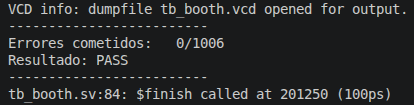
\includegraphics[width=0.5\linewidth]{Figuras/booth_print.png}
    \caption{Resultado impreso del multiplicador \textit{Booth}.}
    \label{fig:booth_print}
\end{figure}

\begin{figure}[H]
    \centering
    \begin{minipage}{\linewidth}
        \centering
        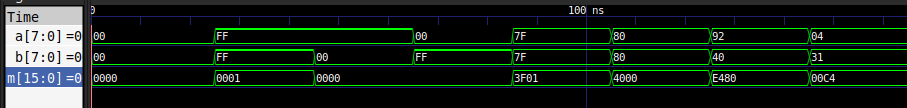
\includegraphics[width=\linewidth]{booth_wave_hex.png}
        \subcaption{En hexadecimal.}
        \label{fig:booth_wave_hex}
    \end{minipage}
    
    \vspace{20px}
    
    \begin{minipage}{\linewidth}
        \centering
        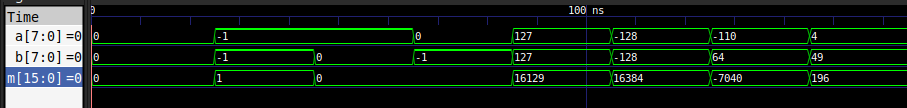
\includegraphics[width=\linewidth]{booth_wave_dec.png}
        \subcaption{En decimal con signo.}
        \label{fig:booth_wave_dec}
    \end{minipage}
    \caption{Formas de onda del multiplicador \textit{Booth radix-2}.}
    \label{fig:booth_wave}
\end{figure}

Como se mencionó anteriormente, la cantidad de productos parciales a utilizar no cambia en este método comparado con un \emph{array multiplier}, pero el tiempo de propagación sí puede ser menor, ya que no se toman en cuenta los carrys en las sumas. De todas formas, se puede realizar el método \textit{Booth radix-4} donde se evalúa el multiplicador cada $3$ bits, permitiendo reducir la cantidad de filas a $N_{bits}/2$. Esto no quiere decir que este método sea el doble de rápido respecto del radix-2, ya que requiere lógica adicional para la decodificación de los $3$ bits y los desplazamientos adicionales.



\section{Conclusiones}                                              \label{sec_3}
El desarrollo de estos ejercicios evidencia los \textit{trade-offs} entre área, velocidad y eficiencia en el diseño lógico digital. Mientras que las arquitecturas puramente jerárquicas o secuenciales, como el \textit{RCA} o el multiplicador \textit{Shift and Add}, resultan sumamente eficientes en el uso de recursos de \textit{hardware} (siendo ideales para sistemas de bajo consumo), topologías más avanzadas como el \textit{CLA}, \textit{CSLA} o los arreglos combinacionales logran reducir significativamente el camino crítico y maximizar el \textit{throughput} a costa de una mayor complejidad y área. De este modo, queda demostrado que no existe una única solución ideal, sino que la elección de la estructura aritmética dependerá estrictamente de las restricciones de frecuencia máxima y recursos disponibles que exija la aplicación final.



\newpage
\nocite{*}
\printbibliography[heading=bibintoc, title={4. \ Referencias}]

\end{document}